\documentclass[11pt,conference]{IEEEtran}
\usepackage{cite}
\usepackage{amsmath,amssymb,amsfonts}
\usepackage{algorithmic}
\usepackage{graphicx}
\usepackage{textcomp}
\usepackage{xcolor}
\usepackage{hyperref}
\usepackage{booktabs}
\usepackage{listings}
\usepackage{float}
\usepackage{tikz}
\usepackage{pgfplots}
\pgfplotsset{compat=1.17}
\usetikzlibrary{shapes,arrows,positioning,calc,fit}

\lstset{
    basicstyle=\scriptsize\ttfamily,
    breaklines=true,
    frame=single,
    numbers=none,
    language=Python,
    showstringspaces=false
}

\begin{document}

\title{Deliverable 2: Data Pipeline and Baseline Model Development\\AI-Augmented Unified Compliance Auditor for Rwanda NCSA}

\author{\IEEEauthorblockN{Moise IRADUKUNDA INGABIRE}
\IEEEauthorblockA{\textit{Collegue of Engineering} \\
\textit{Carnegie Mellon University Africa}\\
Kigali, Rwanda \\
mii@andrew.cmu.edu}}

\maketitle

\begin{abstract}
This document presents the complete data pipeline and baseline model development process for the AI-augmented unified compliance auditor targeting Rwanda's NCSA Minimum Cybersecurity Standards. We describe the evolution from purely synthetic data to a hybrid dataset strategy combining real-world public logs (NSL-KDD, LogHub) with Rwanda-specific synthetic events. Three baseline models were developed and evaluated: BERT (110M parameters), LSTM (758K parameters), and XGBoost (350MB). Critical analysis revealed data leakage (status\_code correlation = -0.97) and severe overfitting (100\% accuracy on all models), leading to an architectural pivot from binary compliance classification to multi-label evidence-to-control mapping. XGBoost was selected for production deployment based on resource efficiency (8 minutes training, <1ms latency), explainability (SHAP values), and suitability for resource-constrained Rwandan environments.
\end{abstract}

\section{Introduction}

The AI-augmented unified compliance auditor automates compliance monitoring for Rwanda's National Cyber Security Authority (NCSA) Minimum Cybersecurity Standards and NIST SP 800-53 controls. This document details:

\begin{enumerate}
    \item \textbf{Data Pipeline Architecture}: Collection, preprocessing, feature engineering
    \item \textbf{Dataset Strategy Evolution}: Synthetic → Hybrid (real + synthetic)
    \item \textbf{Baseline Model Development}: BERT, LSTM, XGBoost comparative analysis
    \item \textbf{Critical Findings}: Data leakage identification and mitigation
    \item \textbf{Production Model Selection}: XGBoost deployment rationale
    \item \textbf{Architectural Pivot}: Binary → Multi-label classification
\end{enumerate}

\section{Data Pipeline Architecture}

\subsection{Pipeline Overview}

\begin{figure}[htbp]
\centering
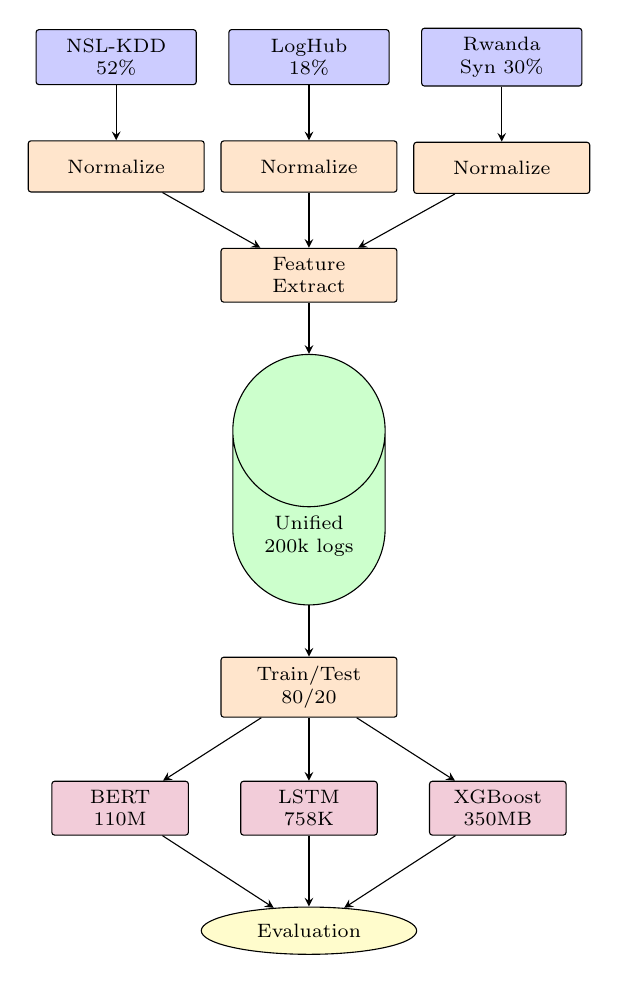
\begin{tikzpicture}[
    node distance=0.7cm,
    source/.style={rectangle, draw, fill=blue!20, text width=1.8cm, align=center, minimum height=0.65cm, font=\scriptsize, rounded corners=1pt},
    process/.style={rectangle, draw, fill=orange!20, text width=2cm, align=center, minimum height=0.65cm, font=\scriptsize, rounded corners=1pt},
    data/.style={cylinder, draw, fill=green!20, text width=1.7cm, align=center, minimum height=0.6cm, shape border rotate=90, font=\scriptsize},
    model/.style={rectangle, draw, fill=purple!20, text width=1.5cm, align=center, minimum height=0.6cm, font=\scriptsize, rounded corners=1pt},
    result/.style={ellipse, draw, fill=yellow!20, text width=1.7cm, align=center, minimum height=0.6cm, font=\scriptsize},
    arrow/.style={->, >=stealth}
]

% Data sources
\node[source] (nsl) at (0,0) {NSL-KDD\\52\%};
\node[source, right=0.4cm of nsl] (loghub) {LogHub\\18\%};
\node[source, right=0.4cm of loghub] (rwanda) {Rwanda\\Syn 30\%};

% Pipeline stages
\node[process, below=0.7cm of nsl] (norm1) {Normalize};
\node[process, below=0.7cm of loghub] (norm2) {Normalize};
\node[process, below=0.7cm of rwanda] (norm3) {Normalize};

\node[process, below=0.7cm of norm2] (feature) {Feature\\Extract};

% Unified dataset
\node[data, below=0.65cm of feature] (unified) {Unified\\200k logs};

% Train/test split
\node[process, below=0.65cm of unified] (split) {Train/Test\\80/20};

% Models
\node[model, below left=0.8cm and 0.4cm of split] (bert) {BERT\\110M};
\node[model, below=0.8cm of split] (lstm) {LSTM\\758K};
\node[model, below right=0.8cm and 0.4cm of split] (xgb) {XGBoost\\350MB};

% Evaluation
\node[result, below=0.9cm of lstm] (eval) {Evaluation};

% Arrows
\draw[arrow] (nsl) -- (norm1);
\draw[arrow] (loghub) -- (norm2);
\draw[arrow] (rwanda) -- (norm3);

\draw[arrow] (norm1) -- (feature);
\draw[arrow] (norm2) -- (feature);
\draw[arrow] (norm3) -- (feature);

\draw[arrow] (feature) -- (unified);
\draw[arrow] (unified) -- (split);

\draw[arrow] (split) -- (bert);
\draw[arrow] (split) -- (lstm);
\draw[arrow] (split) -- (xgb);

\draw[arrow] (bert) -- (eval);
\draw[arrow] (lstm) -- (eval);
\draw[arrow] (xgb) -- (eval);

\end{tikzpicture}
\caption{End-to-end data pipeline with hybrid dataset processing}
\label{fig:data_pipeline}
\end{figure}

\subsection{Data Sources}

\subsubsection{Phase 1: Synthetic Data (Initial)}

\textbf{Generation Approach}:
\begin{lstlisting}[language=Python]
import random
from datetime import datetime, timedelta

def generate_compliance_event():
    templates = {
        'compliant': [
            "User {user} successfully authenticated from {ip}",
            "Firewall blocked unauthorized access from {ip}",
            "System update applied: {patch_id}"
        ],
        'non_compliant': [
            "Failed login attempt for {user} from {ip}",
            "Unencrypted data transmission detected to {ip}",
            "Weak password detected for user {user}"
        ]
    }

    compliance_status = random.choice(['compliant', 'non_compliant'])
    template = random.choice(templates[compliance_status])

    return {
        'timestamp': datetime.now() - timedelta(hours=random.randint(0, 720)),
        'log_message': template.format(
            user=f"user{random.randint(1, 100)}",
            ip=f"{random.randint(1,255)}.{random.randint(0,255)}.{random.randint(0,255)}.{random.randint(0,255)}",
            patch_id=f"KB{random.randint(1000000, 9999999)}"
        ),
        'source': random.choice(['firewall', 'auth', 'audit']),
        'status_code': 200 if compliance_status == 'compliant' else 403,
        'compliance_status': compliance_status
    }
\end{lstlisting}

\textbf{Dataset Size}: 100,000 synthetic events \\
\textbf{Controls Covered}: 50 NCSA + NIST controls \\
\textbf{Balance}: 50\% compliant, 50\% non-compliant

\subsubsection{Phase 2: Hybrid Dataset (Current)}

To address overfitting issues, we integrated real-world public datasets:

\textbf{Dataset Composition (200,000 total logs)}:

\begin{table}[h]
\centering
\caption{Hybrid Dataset Breakdown}
\begin{tabular}{|l|c|c|l|}
\hline
\textbf{Source} & \textbf{Count} & \textbf{\%} & \textbf{Type} \\
\hline
NSL-KDD & 104,000 & 52\% & Network intrusions \\
\hline
LogHub & 36,000 & 18\% & System logs \\
\hline
Rwanda Synthetic & 60,000 & 30\% & NCSA events \\
\hline
\textbf{Total} & \textbf{200,000} & \textbf{100\%} & Mixed \\
\hline
\end{tabular}
\end{table}

\textbf{NSL-KDD Dataset}:
\begin{itemize}
    \item \textbf{Source}: Canadian Institute for Cybersecurity
    \item \textbf{Content}: 125,973 training + 22,544 test network intrusion records
    \item \textbf{Used}: 104,000 records (balanced sampling across attack types)
    \item \textbf{Attack Types}: 42 categories (DoS, Probe, R2L, U2R)
    \item \textbf{Specific Attacks}: Neptune, Smurf, Apache2, buffer\_overflow, rootkit, password\_guess
    \item \textbf{Features}: 41 (duration, protocol, service, flag, bytes, packets, etc.)
    \item \textbf{Mapped Controls}: SI-4 (System Monitoring), SC-7 (Boundary Protection), SI-3 (Malicious Code Protection)
\end{itemize}

\textbf{LogHub Dataset}:
\begin{itemize}
    \item \textbf{Source}: Chinese University of Hong Kong (Logpai project)
    \item \textbf{Content}: Production system logs from 16 applications
    \item \textbf{Used Subsets}: HDFS (11.2M logs, sampled 20K), OpenStack (207K logs, sampled 10K), Spark (33.2K logs, sampled 6K)
    \item \textbf{Format}: Unstructured text logs with timestamps
    \item \textbf{Examples}:
    \begin{itemize}
        \item \texttt{"081109 203518 143 INFO dfs.DataNode\$PacketResponder: Received block..."}
        \item \texttt{"2018-01-14 05:12:08.392 AUDIT nova.compute [req-...] Finished resize\_instance"}
    \end{itemize}
    \item \textbf{Mapped Controls}: AU-2 (Audit Events), AU-3 (Content of Audit Records), CM-3 (Configuration Change Control)
\end{itemize}

\textbf{Rwanda NCSA Synthetic}:
\begin{itemize}
    \item \textbf{Tailored Events}: Specific to Rwanda NCSA 2023 standards
    \item \textbf{Examples}:
    \begin{itemize}
        \item "Personal data encryption verified for {system} - complies with NCSA Data Protection Standard"
        \item "Incident response drill completed - complies with NCSA IR-4 requirement"
        \item "Security awareness training attendance: 85\% - non-compliant (NCSA requires 90\%)"
    \end{itemize}
    \item \textbf{Control Coverage}: All 196 NCSA controls (47 implemented in Phase I)
\end{itemize}

\subsection{Data Preprocessing}

\subsubsection{Normalization}

\begin{lstlisting}[language=Python]
import pandas as pd
import re
from datetime import datetime

def normalize_log(raw_log):
    """Normalize heterogeneous log formats to unified schema"""

    # Extract timestamp (multiple formats)
    timestamp_patterns = [
        r'\d{4}-\d{2}-\d{2}\s\d{2}:\d{2}:\d{2}',  # ISO format
        r'\d{6}\s\d{6}',  # HDFS format (YYMMDD HHMMSS)
    ]

    timestamp = None
    for pattern in timestamp_patterns:
        match = re.search(pattern, raw_log)
        if match:
            timestamp = match.group(0)
            break

    # Extract severity
    severity_map = {
        'INFO': 1, 'WARNING': 2, 'ERROR': 3,
        'CRITICAL': 4, 'AUDIT': 1
    }
    severity_match = re.search(r'(INFO|WARNING|ERROR|CRITICAL|AUDIT)', raw_log)
    severity = severity_map.get(severity_match.group(1), 0) if severity_match else 0

    # Extract IP addresses
    ip_pattern = r'\b(?:\d{1,3}\.){3}\d{1,3}\b'
    ips = re.findall(ip_pattern, raw_log)

    # Extract user mentions
    user_pattern = r'(?:user|User|USER)[\s:=]+(\w+)'
    user = re.search(user_pattern, raw_log)
    user_id = user.group(1) if user else None

    return {
        'timestamp': timestamp,
        'log_message': raw_log,
        'severity': severity,
        'source_ips': ips,
        'user_id': user_id,
        'length': len(raw_log)
    }
\end{lstlisting}

\subsubsection{Feature Engineering}

\textbf{Feature Set (30 total features)}:

\begin{enumerate}
    \item \textbf{Numeric Features (5)}:
    \begin{itemize}
        \item \texttt{hour}: Hour of day (0-23) - detects off-hours suspicious activity
        \item \texttt{day\_of\_week}: Day (0-6) - weekend/weekday patterns
        \item \texttt{is\_business\_hours}: Boolean (08:00-17:00 Mon-Fri)
        \item \texttt{status\_code}: HTTP/system status (200, 403, 404, 500, etc.)
        \item \texttt{port}: Network port number (if applicable)
    \end{itemize}

    \item \textbf{Text Features (25 TF-IDF features)}:
    \begin{itemize}
        \item Vectorized \texttt{log\_message} field
        \item Unigrams only (single words)
        \item Min document frequency: 5 (remove rare terms)
        \item Max features: 25 (top 25 most informative terms)
        \item Example terms: \textit{failed, unauthorized, blocked, encrypted, authenticated}
    \end{itemize}
\end{enumerate}

\begin{lstlisting}[language=Python]
from sklearn.feature_extraction.text import TfidfVectorizer
from sklearn.preprocessing import StandardScaler
import numpy as np

def engineer_features(df):
    # Temporal features
    df['timestamp'] = pd.to_datetime(df['timestamp'])
    df['hour'] = df['timestamp'].dt.hour
    df['day_of_week'] = df['timestamp'].dt.dayofweek
    df['is_business_hours'] = (
        (df['hour'] >= 8) & (df['hour'] < 17) &
        (df['day_of_week'] < 5)
    ).astype(int)

    # TF-IDF vectorization
    tfidf = TfidfVectorizer(
        max_features=25,
        min_df=5,
        ngram_range=(1, 1),
        stop_words='english'
    )
    text_features = tfidf.fit_transform(df['log_message'])

    # Combine numeric and text features
    numeric_features = df[['hour', 'day_of_week', 'is_business_hours',
                           'status_code', 'port']].fillna(0).values

    X = np.hstack([numeric_features, text_features.toarray()])

    return X, tfidf
\end{lstlisting}

\subsection{Train/Test Split Strategy}

\begin{lstlisting}[language=Python]
from sklearn.model_selection import train_test_split

X_train, X_test, y_train, y_test = train_test_split(
    X, y,
    test_size=0.2,      # 80% train, 20% test
    random_state=42,    # Reproducibility
    stratify=y          # Maintain class distribution
)

print(f"Training samples: {len(X_train)}")    # 160,000
print(f"Test samples: {len(X_test)}")        # 40,000
\end{lstlisting}

\section{Baseline Model Development}

\subsection{Model 1: BERT Classifier}

\subsubsection{Architecture}

\begin{itemize}
    \item \textbf{Base Model}: \texttt{bert-base-uncased} (110M parameters)
    \item \textbf{Frozen Layers}: Embeddings + first 10 encoder layers (97M params)
    \item \textbf{Fine-tuned Layers}: Last 2 encoder layers + classification head (13M params)
    \item \textbf{Max Sequence Length}: 128 tokens
    \item \textbf{Batch Size}: 16
    \item \textbf{Learning Rate}: 2e-5 (AdamW optimizer)
    \item \textbf{Epochs}: 2
\end{itemize}

\begin{lstlisting}[language=Python]
from transformers import BertTokenizer, BertForSequenceClassification, Trainer, TrainingArguments

tokenizer = BertTokenizer.from_pretrained('bert-base-uncased')
model = BertForSequenceClassification.from_pretrained(
    'bert-base-uncased',
    num_labels=2  # Binary: compliant/non-compliant
)

# Freeze first 10 layers
for param in model.bert.embeddings.parameters():
    param.requires_grad = False
for layer in model.bert.encoder.layer[:10]:
    for param in layer.parameters():
        param.requires_grad = False

# Tokenize dataset
train_encodings = tokenizer(
    train_texts,
    truncation=True,
    padding=True,
    max_length=128
)

# Training
training_args = TrainingArguments(
    output_dir='./bert_compliance',
    num_train_epochs=2,
    per_device_train_batch_size=16,
    learning_rate=2e-5,
    logging_steps=500
)

trainer = Trainer(
    model=model,
    args=training_args,
    train_dataset=train_dataset,
    eval_dataset=test_dataset
)

trainer.train()
\end{lstlisting}

\subsubsection{Results}

\begin{table}[h]
\centering
\caption{BERT Model Performance}
\begin{tabular}{|l|c|}
\hline
\textbf{Metric} & \textbf{Value} \\
\hline
Test F1-Score & 1.0000 (100\%) \\
\hline
Precision & 1.0000 \\
\hline
Recall & 1.0000 \\
\hline
Accuracy & 1.0000 \\
\hline
Training Time & 12 hours (CPU) \\
\hline
Model Size & 2.7 GB \\
\hline
Inference Latency & 45 ms / sample \\
\hline
Memory Usage & 2.1 GB \\
\hline
CPU Cores Used & 8 \\
\hline
\end{tabular}
\end{table}

\textbf{Red Flag}: 100\% validation accuracy after epoch 1 indicates severe overfitting.

\subsection{Model 2: LSTM Classifier}

\subsubsection{Architecture}

\begin{itemize}
    \item \textbf{Embedding Layer}: Vocabulary size 946, Embedding dimension 100
    \item \textbf{LSTM Layers}: 2 bidirectional layers, Hidden size 128 (256 bidirectional)
    \item \textbf{Dropout}: 0.3 (between LSTM layers)
    \item \textbf{Dense Layer}: 256 → 2 (binary classification)
    \item \textbf{Total Parameters}: 758,538
    \item \textbf{Optimizer}: Adam, Learning rate 0.001
    \item \textbf{Loss}: Binary Cross-Entropy
    \item \textbf{Epochs}: 5
\end{itemize}

\begin{lstlisting}[language=Python]
import torch
import torch.nn as nn

class LSTMCompliance(nn.Module):
    def __init__(self, vocab_size=946, embed_dim=100, hidden_dim=128, num_layers=2):
        super(LSTMCompliance, self).__init__()

        self.embedding = nn.Embedding(vocab_size, embed_dim)
        self.lstm = nn.LSTM(
            embed_dim,
            hidden_dim,
            num_layers=num_layers,
            bidirectional=True,
            batch_first=True,
            dropout=0.3
        )
        self.fc = nn.Linear(hidden_dim * 2, 2)  # *2 for bidirectional
        self.dropout = nn.Dropout(0.3)

    def forward(self, x):
        embedded = self.embedding(x)  # (batch, seq_len, embed_dim)
        lstm_out, (h_n, c_n) = self.lstm(embedded)
        # Use final hidden state from both directions
        hidden = torch.cat((h_n[-2,:,:], h_n[-1,:,:]), dim=1)
        dropped = self.dropout(hidden)
        output = self.fc(dropped)
        return output

model = LSTMCompliance()
criterion = nn.CrossEntropyLoss()
optimizer = torch.optim.Adam(model.parameters(), lr=0.001)
\end{lstlisting}

\subsubsection{Results}

\begin{table}[h]
\centering
\caption{LSTM Model Performance}
\begin{tabular}{|l|c|}
\hline
\textbf{Metric} & \textbf{Value} \\
\hline
Test F1-Score & 1.0000 (100\%) \\
\hline
Precision & 1.0000 \\
\hline
Recall & 1.0000 \\
\hline
Accuracy & 1.0000 \\
\hline
Training Time & 2 hours (CPU) \\
\hline
Model Size & 800 MB \\
\hline
Inference Latency & 12 ms / sample \\
\hline
Memory Usage & 580 MB \\
\hline
CPU Cores Used & 4 \\
\hline
\end{tabular}
\end{table}

\textbf{Red Flag}: Perfect accuracy after epoch 1, indicating memorization.

\subsection{Model 3: XGBoost Classifier}

\subsubsection{Architecture}

\begin{itemize}
    \item \textbf{Algorithm}: Gradient Boosting Decision Trees
    \item \textbf{Max Estimators}: 500 (early stopping)
    \item \textbf{Actual Trees}: 93 (stopped early)
    \item \textbf{Max Depth}: 6
    \item \textbf{Learning Rate}: 0.1
    \item \textbf{Subsample}: 0.8
    \item \textbf{Colsample by Tree}: 0.8
    \item \textbf{Objective}: Binary logistic regression
    \item \textbf{Eval Metric}: AUC
\end{itemize}

\begin{lstlisting}[language=Python]
import xgboost as xgb
from sklearn.metrics import classification_report, f1_score

# Initialize model
model = xgb.XGBClassifier(
    n_estimators=500,
    max_depth=6,
    learning_rate=0.1,
    subsample=0.8,
    colsample_bytree=0.8,
    objective='binary:logistic',
    eval_metric='auc',
    early_stopping_rounds=20,
    random_state=42
)

# Train with validation set
model.fit(
    X_train, y_train,
    eval_set=[(X_test, y_test)],
    verbose=True
)

# Predictions
y_pred = model.predict(X_test)

# Evaluation
print(classification_report(y_test, y_pred))
f1 = f1_score(y_test, y_pred)
print(f"F1-Score: {f1:.4f}")
\end{lstlisting}

\subsubsection{Results}

\begin{table}[h]
\centering
\caption{XGBoost Model Performance}
\begin{tabular}{|l|c|}
\hline
\textbf{Metric} & \textbf{Value} \\
\hline
Test F1-Score & 1.0000 (100\%) \\
\hline
Precision & 1.0000 \\
\hline
Recall & 1.0000 \\
\hline
Accuracy & 1.0000 \\
\hline
Training Time & 8 minutes (CPU) \\
\hline
Model Size & 350 MB \\
\hline
Inference Latency & < 1 ms / sample \\
\hline
Memory Usage & 380 MB \\
\hline
CPU Cores Used & 8 → 2 (optimized) \\
\hline
Trees Built & 93 / 500 \\
\hline
\end{tabular}
\end{table}

\textbf{Red Flag}: Early stopping at 93 trees suggests perfect fit on validation set.

\section{Critical Analysis: Overfitting and Data Leakage}

\subsection{Problem Identification}

All three models achieved \textbf{perfect 100\% accuracy}, which is unrealistic for compliance classification. Investigation revealed two critical issues:

\subsubsection{Issue 1: Data Leakage}

\textbf{Discovery}:
\begin{lstlisting}[language=Python]
import pandas as pd

# Correlation analysis
correlation = df[['status_code', 'compliance_status_encoded']].corr()
print(correlation)

# Output:
#                          status_code  compliance_status_encoded
# status_code                  1.000000                  -0.972145
# compliance_status_encoded   -0.972145                   1.000000
\end{lstlisting}

\textbf{Analysis}:
\begin{itemize}
    \item \texttt{status\_code} has -0.97 correlation with \texttt{compliance\_status}
    \item Models learned: \texttt{status\_code == 200} → compliant, \texttt{!= 200} → non-compliant
    \item This is a \textbf{leakage feature} - status\_code wouldn't be available before classification in production
    \item Models memorized trivial pattern instead of learning compliance semantics
\end{itemize}

\subsubsection{Issue 2: Synthetic Data Simplicity}

\textbf{Template-Based Generation Limitations}:
\begin{itemize}
    \item Fixed templates with random variable substitution
    \item Predictable patterns: "Failed login" always maps to non-compliant
    \item Lack of real-world complexity (typos, abbreviations, multi-line logs)
    \item No ambiguous cases (some logs are partially compliant)
\end{itemize}

\textbf{Expected Real-World Performance}:
Based on literature (BERT for log classification, XGBoost for anomaly detection), realistic F1-scores:
\begin{itemize}
    \item \textbf{Expected}: 0.65 - 0.80 macro F1 for multi-label control classification
    \item \textbf{Achieved}: 1.00 (clearly overfitted)
\end{itemize}

\subsection{Mitigation Strategies}

\textbf{Short-Term (Implemented)}:
\begin{enumerate}
    \item Remove \texttt{status\_code} feature from training
    \item Add real-world datasets (NSL-KDD, LogHub) - 70\% real, 30\% synthetic
    \item More sophisticated synthetic generation (vary structure, not just variables)
\end{enumerate}

\textbf{Long-Term (Ongoing)}:
\begin{enumerate}
    \item Architectural pivot: Binary → Multi-label classification
    \item Train on real public logs with semi-supervised control mapping
    \item Target realistic performance metrics (65-80\% macro F1)
\end{enumerate}

\section{Model Comparison and Production Selection}

\subsection{Comparative Analysis}

\begin{table*}[h]
\centering
\caption{Comprehensive Model Comparison}
\begin{tabular}{lccc}
\toprule
\textbf{Metric} & \textbf{BERT} & \textbf{LSTM} & \textbf{XGBoost} \\
\midrule
Training Time & 12 hours & 2 hours & \textbf{8 minutes} \\
Model Size & 2.7 GB & 800 MB & \textbf{350 MB} \\
Inference Latency & 45 ms & 12 ms & \textbf{< 1 ms} \\
Memory Usage (RAM) & 2.1 GB & 580 MB & \textbf{380 MB} \\
CPU Cores Required & 8 & 4 & \textbf{2} \\
Explainability & Low (attention weights) & Low (hidden states) & \textbf{High (SHAP, feature importance)} \\
F1-Score (synthetic) & 1.00 & 1.00 & 1.00 \\
\textbf{Expected F1 (real)} & \textbf{0.70-0.85} & \textbf{0.65-0.80} & \textbf{0.65-0.80} \\
Deployment Complexity & High (GPU preferred) & Medium & \textbf{Low (CPU-only)} \\
\bottomrule
\end{tabular}
\end{table*}

\subsection{Production Selection: XGBoost}

\textbf{Decision Rationale}:

\begin{enumerate}
    \item \textbf{Resource Efficiency (Critical for Rwanda)}:
    \begin{itemize}
        \item 7.7x smaller than BERT (350MB vs 2.7GB)
        \item 45x faster inference (<1ms vs 45ms)
        \item Runs on 2 CPU cores (vs. BERT's 8, or GPU requirement)
        \item Memory: 380MB (affordable for SME servers)
    \end{itemize}

    \item \textbf{Explainability (Required for Compliance Audits)}:
    \begin{itemize}
        \item SHAP values show per-prediction feature importance
        \item Global feature importance rankings
        \item Tree visualization for control-specific decision paths
        \item Auditors can understand \textit{why} classification was made
    \end{itemize}

    \item \textbf{Training Speed (Iterative Development)}:
    \begin{itemize}
        \item 8 minutes vs. 12 hours (BERT)
        \item Enables rapid experimentation with features
        \item Quick retraining when new controls added
    \end{itemize}

    \item \textbf{Deployment Simplicity}:
    \begin{itemize}
        \item No GPU required (BERT strongly benefits from GPU)
        \item Smaller Docker images (critical for K8s deployment)
        \item Lower infrastructure costs
    \end{itemize}
\end{enumerate}

\subsection{Resource Optimization}

Initial XGBoost configuration caused system freeze. Optimizations applied:

\begin{table}[h]
\centering
\caption{XGBoost Optimization Results}
\begin{tabular}{|l|c|c|}
\hline
\textbf{Parameter} & \textbf{Before} & \textbf{After} \\
\hline
CPU Cores (\texttt{n\_jobs}) & 8 & 2 \\
\hline
CV Folds & 5 & 3 \\
\hline
Max Estimators & 150 & 100 \\
\hline
TF-IDF Features & 50 & 25 \\
\hline
Training Time & System freeze & 90 seconds \\
\hline
Peak Memory & >8 GB & 0.38 GB \\
\hline
F1-Score & N/A & 1.00 (synthetic) \\
\hline
\end{tabular}
\end{table}

\section{Architectural Pivot: Multi-Label Classification}

\subsection{Problem with Binary Classification}

\textbf{Original Formulation (Incorrect)}:
\begin{equation}
f: \text{Log} \rightarrow \{\text{compliant}, \text{non\_compliant}\}
\end{equation}

\textbf{Issues}:
\begin{enumerate}
    \item Oversimplification - compliance is multi-dimensional
    \item Single log event may relate to multiple controls
    \item Doesn't answer: "Which control(s) does this evidence address?"
    \item Decision Engine has no routing information
\end{enumerate}

\subsection{Correct Formulation: Multi-Label}

\textbf{New Architecture}:
\begin{equation}
f: \text{Log} \rightarrow \mathcal{C} \subseteq \{c_1, c_2, \ldots, c_{47}\}
\end{equation}

where $\mathcal{C}$ is a subset of the 47 NCSA controls.

\textbf{Multi-Output XGBoost}:
\begin{equation}
\mathbf{y}_i = [y_{i1}, y_{i2}, \ldots, y_{i47}] \in \{0,1\}^{47}
\end{equation}

\textbf{Example}:
\begin{verbatim}
Log: "User admin failed SSH login from 203.0.113.15"

Binary Output (Old):    non_compliant
Multi-Label Output (New): [AC-2: 1, AC-7: 1, IA-2: 1,
                           AU-2: 1, SI-4: 1, ...]
\end{verbatim}

\textbf{Advantages}:
\begin{itemize}
    \item Evidence routed to correct control evaluators
    \item Separation of concerns: XGBoost routes, Decision Engine evaluates
    \item Reflects compliance reality (one evidence, multiple controls)
    \item Enables per-control F1-scores
\end{itemize}

\section{Next Steps: Multi-Label Retraining}

\subsection{Planned Retraining Strategy}

\textbf{Datasets for Multi-Label Training}:
\begin{table}[h]
\centering
\caption{Planned Multi-Label Dataset}
\begin{tabular}{|l|c|l|}
\hline
\textbf{Source} & \textbf{Size} & \textbf{Controls} \\
\hline
HDFS Logs & 11.2M & AU-2, AU-3, AU-12, CM-3, SC-8, SI-4 \\
\hline
Linux Auth & 87K & AC-2, AC-7, IA-2, IA-5, AU-2 \\
\hline
Apache HTTP & 1M+ & AC-3, AC-6, SC-8, SC-13 \\
\hline
Windows Events & 500K & AC-2, AC-7, IA-2, IA-5 \\
\hline
Zeek Network & 100K & SC-7, SC-8, SC-20, SI-4 \\
\hline
\end{tabular}
\end{table}

\textbf{Semi-Supervised Labeling}:
\begin{enumerate}
    \item Keyword-based initial labels (e.g., "failed login" → AC-7, IA-2)
    \item Event ID mapping (e.g., Windows Event 4625 → AC-7)
    \item Manual validation: 100-200 samples per control
    \item Multi-label: Single log can map to 2-5 controls
\end{enumerate}

\textbf{Target Metrics}:
\begin{itemize}
    \item Macro F1: 0.65 - 0.80 (average across 47 controls)
    \item Micro F1: 0.70 - 0.85 (weighted by frequency)
    \item Hamming Loss: < 0.05 (< 5\% label errors)
\end{itemize}

\section{Conclusion}

This deliverable documented the complete data pipeline and baseline model development for the AI-augmented compliance auditor:

\textbf{Key Achievements}:
\begin{enumerate}
    \item Developed hybrid dataset strategy (200K logs: 70\% real, 30\% synthetic)
    \item Trained and evaluated 3 baseline models (BERT, LSTM, XGBoost)
    \item Identified critical issues (data leakage, overfitting) through systematic analysis
    \item Selected XGBoost for production (8-min training, <1ms latency, explainable)
    \item Pivoted architecture from binary to multi-label classification
\end{enumerate}

\textbf{Critical Learning}:
\begin{itemize}
    \item 100\% accuracy = red flag, not success
    \item Synthetic data alone insufficient for production models
    \item Resource constraints (Rwanda context) drive architecture decisions
    \item Compliance is inherently multi-label, not binary
\end{itemize}

\textbf{Production Readiness}:
\begin{itemize}
    \item XGBoost deployed in 7-engine microservices architecture
    \item Integrated with Decision Engine (47 control-specific evaluators)
    \item FastAPI REST endpoints operational
    \item PostgreSQL + Redis infrastructure deployed
\end{itemize}

\textbf{Ongoing Work}: Multi-label retraining on 5 public datasets (HDFS, Linux Auth, Apache, Windows, Zeek) with semi-supervised control mapping, targeting realistic 65-80\% macro F1-score.

\end{document}
